
\documentclass[10pt, conference, compsocconf]{IEEEtran}

\ifCLASSINFOpdf
  \usepackage[pdftex]{graphicx}
  % declare the path(s) where your graphic files are
  \graphicspath{{./images/}}
  % and their extensions so you won't have to specify these with
  % every instance of \includegraphics
  \DeclareGraphicsExtensions{.pdf,.jpeg,.png,.jpg}
\else
  % or other class option (dvipsone, dvipdf, if not using dvips). graphicx
  % will default to the driver specified in the system graphics.cfg if no
  % driver is specified.
  \usepackage[dvips]{graphicx}
  % declare the path(s) where your graphic files are
  \graphicspath{{./images/}}
  % and their extensions so you won't have to specify these with
  % every instance of \includegraphics
  \DeclareGraphicsExtensions{.eps}
\fi

% correct bad hyphenation here
\hyphenation{op-tical net-works semi-conduc-tor}


\begin{document}
%
% paper title
% can use linebreaks \\ within to get better formatting as desired
\title{Usage Management of Personal Medical Records}


% author names and affiliations
% use a multiple column layout for up to two different
% affiliations
\author{\IEEEauthorblockN{Christopher C. Lamb, Pramod A. Jamkhedkar, Gregory L. Heileman, Ravi K. Kadaboina}
\IEEEauthorblockA{University of New Mexico\\
Department of Electrical and Computer Engineering\\
Albuquerque, NM 87131-0001 \\
\{cclamb, pramod54, heileman, ravik\}@ece.unm.edu}
}

% conference papers do not typically use \thanks and this command
% is locked out in conference mode. If really needed, such as for
% the acknowledgment of grants, issue a \IEEEoverridecommandlockouts
% after \documentclass

% for over three affiliations, or if they all won't fit within the width
% of the page, use this alternative format:
% 
%\author{\IEEEauthorblockN{Michael Shell\IEEEauthorrefmark{1},
%Homer Simpson\IEEEauthorrefmark{2},
%James Kirk\IEEEauthorrefmark{3}, 
%Montgomery Scott\IEEEauthorrefmark{3} and
%Eldon Tyrell\IEEEauthorrefmark{4}}
%\IEEEauthorblockA{\IEEEauthorrefmark{1}School of Electrical and Computer Engineering\\
%Georgia Institute of Technology,
%Atlanta, Georgia 30332--0250\\ Email: see http://www.michaelshell.org/contact.html}
%\IEEEauthorblockA{\IEEEauthorrefmark{2}Twentieth Century Fox, Springfield, USA\\
%Email: homer@thesimpsons.com}
%\IEEEauthorblockA{\IEEEauthorrefmark{3}Starfleet Academy, San Francisco, California 96678-2391\\
%Telephone: (800) 555--1212, Fax: (888) 555--1212}
%\IEEEauthorblockA{\IEEEauthorrefmark{4}Tyrell Inc., 123 Replicant Street, Los Angeles, California 90210--4321}}

% make the title area
\maketitle


\begin{abstract}
Personal medical record (PMR) management is under new scruitiny as private companies move into the market and government agencies actively address percieved health care distribution inequalities and inefficiencies.  Current systems are coarse-grained and provide consumers very little actual control over their data.  Herein, we propose an alternative system for managing the use of healthcare infomormation.  This system is finer grained, allows for data mining and repackaging, and gives users more control over their data, allowing it to be distributed to their specifications.  In this paper, we outline the characteristics of such a system in different contexts, present relavant background information and research leading to the system design, and cover specific usage scenarios supported by this system that are difficult to control using simpler access control strategies.
\end{abstract}

\begin{IEEEkeywords}
%component; formatting; style; styling;
usage management; electronic medical records

\end{IEEEkeywords}


% For peer review papers, you can put extra information on the cover
% page as needed:
% \ifCLASSOPTIONpeerreview
% \begin{center} \bfseries EDICS Category: 3-BBND \end{center}
% \fi
%
% For peerreview papers, this IEEEtran command inserts a page break and
% creates the second title. It will be ignored for other modes.
\IEEEpeerreviewmaketitle

\section{Introduction}
% no \IEEEPARstart
New healthcare legislation has spurred previously unknown levels of public and private investment in technologies supporting more efficient healthcare delivery \cite{Emr:Web:Recovery}.   An active area of examination is electronic health records.  Current systems, such as Microsoft HealthVault and Google Health are a start in this area, but provide rudimentary control over health information, provide consumers with very little actual control of their information, and essentially demand proprietary lockin to these products because of the amount of effort involved with data transfer \cite{Emr:EvaluationHealthInf}.

We propose an open, consumer-centric approach to health information storage and consumption centered around flexible and fine-grained usage management policies.  User empowering systems in this area are needed to allow users control over the information that represents them, and would be in high demand if appropriately designed \cite{Emr:PyAmWaCr}.  We propose to address this need by bundling health information (either entire records or subsets of records) with traceable and aggregateable usage policies controlled by the users themselves.  Users would have the ability to make aspects of their records available to everyone from research institutions looking for historical information for studies, to specific healthcare providers who need specific information to support diagnoses.  Furthermore, institutions would be able to combine information from groups of users and determine dynamically via policy evaluation how that new set of data can be used in a way that complies with all included user policies.  If the combined dataset cannot be used, policies can be analyzed to determine the cause of the policy conflict.

We propose, design, and demonstrate a system that supports granular management of the data elements of an electronic medical record.  This management will allow users to specify policies over the data itself rather than the entire record in question, providing control over information dissemination.  We will demonstrate this control in three distinct scenarios.  The first will include two distinct parties negotiating over access to specific information contained in a medical record.  If the parties can reach an agreement, the information consumer will be granted access to specific medical data, for an agreed-upon price.  The second demostrates a data broker combining a set of previously acquired medical record data into an aggregate set for research, if the licensure is in fact compliant between all selelected data elements.  Finally, the aggregated data set will be placed back into the market.

This kind of system, allowing users control over their data in ways fostering ease of dissemination, use and reuse, helps users receive better, more targed care, helps providers easly access required information, and allows this kind of data to be more easily examined and mined.  We use established system design principles, used in the develoment of internet-scale networks to create a open flexible system \cite{Al:04,BlCl:01,ClWrSoBr:02}.  We standardize certain features, such as operational semantics and ontological domains, but otherwise limit the impact of the policy system on data dissemination as much as possible.

% Usage Management info goes here

\subsection{Previous Work}
Past research applicable to this area includes usage management, digital rights management (DRM), and access control.  Most of the research applicable to the combination of previous arfifacts into a single aggregate artifact comes from the DRM world in particular.  Generally, these expressive languages have been fundamentally based on different types of mathematical logic or formalisms with reasoning capabilities \cite{ArHu:07,BaMi:06,ChCoEtHaJoLa:03,HaWe:04,HaWe:08,PuWe:02,XiBjFu:08}.  This approach, while useful in closed systems, tends to not work as usefully in more open dynamic environments.  This has led to the development of translation mechanisms to address interoperability needs \cite{HeJa:05,PoPrDe:04,ScTaWo:04}.  This translation process is difficult for most policy languages, and in fact infeasible as a result \cite{KoLaMaMi:04,SaShUe:04}.  Alternative approaches have required the use of sophiticated and powerful languages that must be adopted as a universal standard \cite{OMADRM,ODRL-req,Wa:04,XrML-spec}.  This approach inherently limits innovation and flexibility \cite{HeJa:05,JaHe:04,JaHe:08,JaHeMa:06}.

\section{New Models}
Engineers and futurists have speculated as to the impact of personal medical records for years \cite{Emr:Web:BestCaseEMR,Emr:Web:WorstCaseEMR}.  Others have speculated on the institutional use of personal medical records by organizations in today's regulated medical environment \cite{Emr:doi:10.1056/NEJMc081118}.  Health records, when under the control of the person they address, are no longer controlled by the Health Insurance Portability and Accountability Act (HIPPA), though the companies that manage them on the user's behalf in these cases are regulated in most aspects by the Electronic Communications Privacy Act \cite{Emr:doi:10.1056/NEJMsb0800220}.  In total, These concerns imply certain requirements on robust medical record systems, making use models and record control more complex.  None of the promises or concerns of personal medical records can be realized or mitigated without strong usage management.  With a dependable usage management capability, personal medical records open new horizons in the services landscape for interested adopters.

\subsection{A Note on Reliability}
%Consumer, physician(s) (primary, emergency, etc.); editability constraints; auditing
In order for PMRs to be effective, they must be actively used by health care providers.  A system with the wrong kinds of editability constraints or auditing capabilities is at risk of remaining unused by an individual's care providers.  Ideally, these kinds of health records would contain the kind of information a physician would include in a patient's chart.  Providers are required to maintain this is information for adequate patient treatment.  If this information can be arbitrarily edited however, it loses it's credibility.

In fact, many employer-sponsored monitoring programs may incentivize gold-plating medical histories.  Systems like Virgin HealthMiles are marketing themselves directly to employers as ways to monitor employee health. \cite{Emr:Web:VirginHealthMiles}.  Companies are using Virgin HealthMiles to track employee exercise, and as an incentive to use the product (and get more exercise), are offering additional contributions to employer-sponsored health savings accounts if employees meet certain criteria.  Similar senarios could be right around the corner for personal health management systems, were employers incentivize employees to decrease blood pressure, change diet, or similar kinds of things.  In those situations, the pressure for users to alter their records to reflect the reality their employers want to see will be immense, and many users are likely to resort to embellishing their records as a result. Once that happens, health care providers can no longer use the records to provide care.

Any system managing these kinds of records must therefore provide mechanisms to certify, if not the accuracy of the provided information, at least the veracity of it.  Care providers must be able to trust the information provided in a given record, and must not be required to shoulder the burden of viewing the record's edit history in order to do so.  This implies a separation of roles between those who can edit the content of a given record, and those who control how the content of that record may be used.

\subsection{Remote Information Access}
% Travel, schools, immigration:
% who are the players?
% what do they need access to?
% why?
% when do they need it?
% where are the players physically located?
% how would this happen with PMR? Describe system; use scenario
% address pro/con whereever appropriate
Remote access to a patient's health care information is a standard feature of everyday life to which most of us pay little attention.  While in school, we are required to provide evidence of vaccination.  When older, travel to most parts of the world requires rounds of injections.  Most travellers are strongly advised to purchase additional travel insurance to ensure appropriate care in emergencies.  Certainly, when travelling to some parts of the world internet access can be difficult to acquire, but nevertheless such access is much more common now than it was even two years ago, and is becoming easier and easier to find with the proliferation of cellular telephone networks in hertofore undeveloped countries.  

Open access to this kind of healhcare information would certainly make these scenarios easier to deal with for any user, but require strong usage management protections to be effective.  In each case we have distinct sets of users that require access to care information, and in each case those users require access to a specific and limited sections of a personal healthcare record.  School adminstrators, for example, need to confirm the vaccination status of students.  This requires unfettered access to a student's vaccination history, but not to that student's psychiatric care or genetic record.  Likewise, travel visa providers may need access to similar information.  On the other hand, care providers no matter the country of origin require comprehensive care record access in order to provide timely and accurate care.  Furthermore, users have different requirements with respect to the speed of access.  School adminstrators have much less of an urgent, pressing need for care information that an Ethiopian doctor treating an injured patient.  

Importantly, access need not be granted permanently.  Both administrators and foriegn care providers could be given general role-based access that can be removed when no longer neccessary.

The ability to provide care information in a secure, manageable way in these scenarios saves users significant time and headache.  Rounding up and delivering vaccination records to school adminstrators is time consuming and stressful.  Receiving emergency health care in foriegn countries is more than a little frightening.  Systems that can help ameliorate these kinds of situations would certainly be useful.  Furthermore, without specific controls over specific data elements composing a given record, these users cannot be appropriately limited in their access.

\subsection{Monitoring}
% Ongoing health monitoring
% who would use this and why?
% what do they want to see?
% when? what are the implications of that?
% how would this happen? is it coersive? describe system; use scenario
% more pro/con
To constrain health care costs, some employers are beginning to implement holistic preventative health programs.  These programs are structured to attempt to lower overall healthcare costs for a large group of employees through regular screenings, exercise programs, and key health marker monitoring.  Employers are interested in monitoring indicators like trigyceride levels, serum cholesterol, HDL/LDL ratios, blood glucose, blood pressure, and the like.  Employee participation is not neccessarily mandated, but can be encouraged through additional contributions to health savings accounts for participating employees.  In these cases, employers have specific things in which they have an interest. Employees on the other hand likely have information in their care records they very much want to keep out of their employers hands.  For example, an employee may very much want the additional HSA contribution for her family, but is not inclined to let her employer know about her anti-depression medications or her recent treatment for alcohol dependency.

A dependable usage management system supports this kind of partitioned use.  With appropriate controls, this information can be centralized and controlled by the record owner, who can create limited access for employers.  Furthermore, this kind of information can be aggregated by the user over a period of years, demonstrating a pattern of healthy behavior, and perhaps making that record owner more attractive to future employers.  Sensitive information can still be controlled by limiting access.

\subsection{Custom Care}
When users have aggregated medical information at a single location, companies can now access infomormation ranging from previous drug reactions, current prescription status, and the current state of any disease markers.  Users can also make any reactions to medications known essentially immediately, rather than having to wait until able to visit a particular physician.  This kind of information could allow pharmaceutical companies to offer innovative services tailoring medications specifically for individual needs.  For example, large doses of Niacin are common treatment for patients with high serum cholesterol characterised by low HDL and high LDL.  One of the unfortunate side effects of Niacin is facial flushing \cite{Emr:Web:Niacin}.  This is a common but by no means universal side effect of Niacin use.  It can be alleviated in many cases by ingesting Aspirin 20-30 minutes prior to taking niacin \cite{Emr:Web:Niacin}.  Patients that suffer from this particular side effect could have their dose customized and time-released to relieve this discomfort, but only of pharmeceutical providers know this is a patient's problem.

This kind of system promises to provide more responsive care at a potentially lower cost to patients, as long as patient data is available to custom medication providers.  A usage management scheme controlling specific information with respect to pharmeceutical providers could allow those providers to create custom medications for clients  better suited to those specific users.
% Custom pharma
% What exactly is this, and why would users care?
% how would it work?
% who would use it?
% describe system; use scenario
% pro/con

\subsection{Data Marketplace}
%Wherever Times is specified, Times Roman or Times New Roman may be used. If neither is available on your system, please use the font closest in appearance to Times. Avoid using bit-mapped fonts if possible. True-Type 1 or Open Type fonts are preferred. Please embed symbol fonts, as well, for math, etc.
The system we describe in the following sections incorporates a market to allow users and brokers to profit from the use of electronic medical data released under mutually acceptable terms, where usage policies accompany filtered data for either dynamic or static evaluation.  Usage policies themselves are essentially unlimited in how they describe the use of a specific medical record.

\section{System Architecture}
Whatever the final technical attributes of this kind of system are, that system must at least embody certain attributes and requirements.  That architecture must furthermore facilitate usage management as a first-order attribute.

\subsection{Requrements and Attributes}
This type of system has a group of attributes and requirments that it must embody in order to fulfil the use secenarios outlined in the previous section.  Without these, the system would either be poorly received by the targed user population or essentially non-functional.  Of course, simply aligning with these features does not guarantee widespread use; they are neccessary, but not sufficient to guarantee widespread adoption.  Core features include:
\begin{itemize}
\item \textit{Editability} When considering a specific medical record, certain fields of that record should be editable by the owner.  Other fields must only be editable by specific medical providers.  The data owner has complete control over who those providers are, as well as what roles they fulfil.  Certain predefined roles however have access to fields of the medical record that the owner does not.  For example, a physician in the provider role is able to add information to a medical record, and edit information that provider has previously entered.  The record owner cannot edit or change that information, but can edit personal contact information.
\item \textit{Roles} The system must have clearly partitioned roles related to ownership of specific areas of a given record.  These roles must be verifiable as well.  For example, someone assigned to a provider role must be verified as a healthcare provider to prevent record owners from creating spoofed accounts to circumvent record protections.
\item \textit{Auditability} The system must be able to keep a clear record of who edited what, what those specific changes were, how they were made, and when.  This audit trail helps to establish the trustworthiness of the system as a whole, and can provide version control like functionality over records.
\item \textit{Security} The system must take advantage of modern security systems as much as possible to provide additional control over assets.  Without providing adequate security, sensitive information could leak to unscrupulous third parties.  For example, a data owner that has been treated for sexually transmitted diseases in the past five years, but has in fact been married for a decade, may want to keep that information as sequestered as possible.
\item \textit{Accessibility} Some of the outlined scenarios directly imply wide accessiblility geographically, while others require access to medical information from devices with a variety of form factors ranging from modern smartphones to tables to desktop computers.  Still others require data to be delivered through data-centric rather than human readable means.  Not providing this kind of open, widely accessible system makes data entry and eventual use prohibitively difficult.
\item \textit{Performance} Core functionality must be high performance.  Data entry must be engaging and responsive, or providers will simply abandon the system for other, more traditional ways of recording user information.  Data retrieval must be likewise snappy, especially in critical care scenarios.
\item \textit{Flexibility} This system and the data it manages can be used in a wide variety of contexts.  In order to remain relevant, it must be flexible enough to be easily integrated with other arbitrary systems in both de-facto (e.g. RESTful access) and officially standardized (e.g. WS-* SOAP-centric access) ways.
\item \textit{Extensibility} It must provide programmatic interfaces to allow integrations with other currently unknown systems.  Not doing so limits how users can access and expoit the information they own.
\end{itemize}
The system as a whole provides management of personal medical records, which must obviously be addressed by any proposed system architecture.  This management includes record creation, read, and update. It should not delete any data healthcare data, but other less sensitive information should be deletable.

Other features like notifications on certain predefined events or predefined integrations with systems like twitter or facebook may certainly be useful, but are not core functionalities the system must provide.  They should be able to be addressed via core extensibility mechanisms and programming interfaces however.  

\subsection{Sample System Architecture}
A potential system architecture fulfilling the currently known attributes and requirements is outlined in Figure ~\ref{fig:RuntimeView}.
\begin{figure}[!t]
\centering
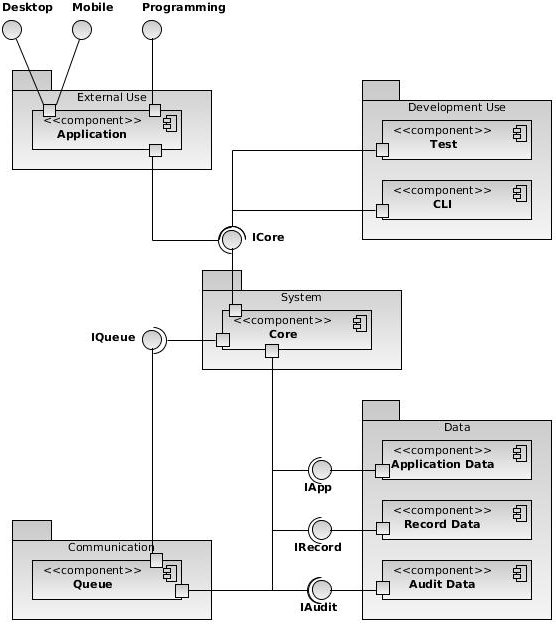
\includegraphics[width=3in]{HisbSystemArch}
\caption{System Architecture Runtime Component View}
\label{fig:RuntimeView}
\end{figure}

\section{Sample System - Data Marketplace}
% Go into what the market is and why we need to use one; describe who would use it and their roles; describe when it would be used and how it could be implemented
Here, we incentivize electronic medical record adoption via the use of a data marketplace.  We have three primary categories of users in mind:

\begin{figure}[!t]
\centering
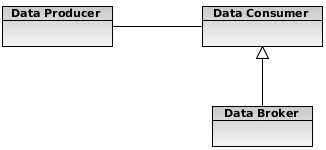
\includegraphics[width=2in]{roles}
\caption{System Roles}
\label{System Roles}
\end{figure}

\begin{itemize}
\item \textit{Data Producers} who produce and market electronic medical information.  This category is generally limited expressly to individual users who require medical care and other related products.
\item \textit{Data Consumers} who directly consume medical information.  This category includes physicians, research institutions, and the like.
\item \textit{Data Brokers} who acquire and remarket medical data from data producers, making that data available in some kind of value-added for to data consumers.  They are a proper subset of data consumers.
\end{itemize}

\textit{Data Producers} would use the medical data market to profit from their personal information.  When negotiating over specifics concerning how their data can be used, they are free to manipulate any aspect of the usage terms prior to a final agreement with a \textit{data consumer}.  The \textit{data consumer} can accept or reject a specific proposal, as can a \textit{data producer}.  A typical negotiation would look something like this:
\begin{enumerate}
\item A \textit{data consumer} searches the marketplace for medical information meeting specific requirements.  This step is a call to a specific search interface in our example, but could be a manual process.
\item The search yields some results.  This proposed system returns a list of contact information of known \textit{data producers} that have data matching the search requirements.
\item The \textit{data consumer} initiates a negotiation for access to specific data.
\begin{enumerate}
\item The \textit{data consumer} contacts the \textit{data producer} and submits and initial proposal.
\item The \textit{data producer} responds to the initial proposal, either be indicating acceptance, rejecting the proposal, or submitting a counter proposal.
\item The \textit{data consumer} is then free to respond with acceptance, rejection, or a counterproposal of her own.
\end{enumerate}
\item Eventually, the negotiation will conclude with the parties having reached an agreement describing access to specific medical data with associated term or having failed to come to mutually acceptable terms with respect to data access.  
\end{enumerate}

Usage terms in a successful conclusion generally describe what the \textit{data consumer} can access, how they may use it and for how long, where it may be accessed, and so on.  It will also usually describe some kind of payment for use, which can be based on any arbitrary number of factors such as time, date, location, attribution, or perhaps in combination with other data.

The market implemented in this system is built around JADE, an open source agent develoment framework based on FIPA agent specifications \cite{Emr:Web:Jade,Emr:Web:Fipa}.

\subsection{System Ontology}
%Describe ontology, describe relationships, define elements; this is a system meta-model; who uses it, what it is (describe/define), why is it important, where, when, how is it used
This system is built around a common ontology that needs must be understood by any system developers.  It is currently used to define relationships and entities within the system at design and run time.  The primary elements in this ontology are:
\begin{itemize}
\item \textit{Producer} This is a data producer as defined in our user model.  A data producer owns a given \textit{record} that has been created over a lifetime of medical care.
\item \textit{Consumer} Again from the user model, a data consumer.  Data consumers use medical data in some way.
\item \textit{Record} A medical record.  We can envision this as a set of discrete medical facts.
\item \textit{Filter} A transformation of a medical record.  If we have a record $ r $, we can transform $ r $ into $ r' $ by applying a transformation $ t $ such that $ r' = t(r) $ where $ t : record \rightarrow record $ and $ r' \subseteq r $.
\item \textit{Filtered Record} A filtered record is a record to which a filter has been applied.  If we have a filtered record $ r' $ derived from a record $ r $, then $ r' \subseteq r $.
\item \textit{License} A license describes the usage policy associated with a given filtered record.  This controls all aspects of filtered record use by an associated consumer.  The specific terms are negotiated over by the producer and the consumer until some optimal consensus is reached, and they then bind the use of an associated filtered record.  Licenses must provide the ability to trace use of transitively associated artifacts regardless of the degree of separation as well.  For example, if we have an artifact $ a $ composed of sets of data elements $ e_{0}, e_{1}, ... , e_{n} $ derived from records $ r_{0}, r_{1}, ... , r_{n} $, we need to be able to ensure that any use of a set of data elements $ e_{i}, i < n $ is within the policy bounds of record $ r_{i}, i < n $ and any compensation associated with such use is correctly attributed to the original data owners and brokers.
\item \textit{Bundle} A filtered record and associated license.  This is distributed to data consumers.
\end{itemize}

\begin{figure}[!t]
\centering
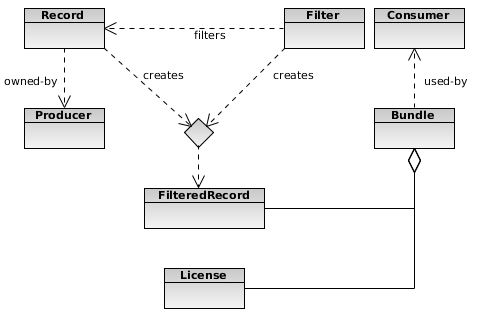
\includegraphics[width=3in]{ontology}
\caption{System Ontology}
\label{System Ontology}
\end{figure}

\subsection{Dynamic and Static Policy Evaluation}
%what who when where why how
%(what) define dynamic and static policy evaluation, elucidate specific advantages/disadvantages of each & where used, go over which we need to use here and why
Usage policies can be evaluated over a spectrum bordered by two distinct approaches - either dynamically, at request time, or statically, when a bundle is created.  Pure dynamic policy evaluation evaluates the entire policy against an artifact at \textit{request time}, specifically and only when a request for an action is made by a consumer.  Static evaluation only occurs when \textit{the bundle is created} and is not evaluated at any later time.  While dynamic policies are more powerful, static policies are generally simpler to define, create, and apply.  Dynamic policy evaluation requires significant runtime infrastructure as well, which static evaluation will never require.  Furthermore, that runtime infrastructure must be present in a variety of systems, implemented upon a myrad of platforms in a slew of different programming languages.  Still, we have compelling reasons for developing dynamic evaluation systems.  Static systems cannot evaluate dynamic properties well.  Attributes like time are impossible to adjudicate with the simplest of static licenses and require some kind of dynamic evaluation.  Likewise, evaluation of a bundle's context is equally impossible to do with simple static policies.  Dynamic policies are more suitable for content that producers are interested in providing for unexpected use, while static policies generally only support predefined use scenarios.

In this system, we propose to use a combination of static and dynamic approaches.  Static policy evaluation occurs immediately after negotiation between the producer and consumer, when a filter is applied to the medical record.  This simplifies dynamic policy requirements by limiting the data that needs to be evaluated after the bundle is released.  If this filter were not applied, the dynamic policy would need to additional clauses to support hiding only those data elements to which the consumer has not been granted access.  All other evaluation occurs after the bundle is delivered to the consumer.  In order to support more complex and unenvisioned usage scenarios, including evaluating usage based on time constraints, this framework provides extensive dynamic evaluation capabilities after the initial filtering phase.  We also need to be able to support seamless operation over protected artifacts while disconnected from any kind of network or communication medium.  These factors lead to a powerful \textit{and local} dynamic policy evaluation system.

% An example of a floating figure using the graphicx package.
% Note that \label must occur AFTER (or within) \caption.
% For figures, \caption should occur after the \includegraphics.
% Note that IEEEtran v1.7 and later has special internal code that
% is designed to preserve the operation of \label within \caption
% even when the captionsoff option is in effect. However, because
% of issues like this, it may be the safest practice to put all your
% \label just after \caption rather than within \caption{}.
%
% Reminder: the "draftcls" or "draftclsnofoot", not "draft", class
% option should be used if it is desired that the figures are to be
% displayed while in draft mode.
%
%\begin{figure}[!t]
%\centering
%\includegraphics[width=2.5in]{myfigure}
% where an .eps filename suffix will be assumed under latex, 
% and a .pdf suffix will be assumed for pdflatex; or what has been declared
% via \DeclareGraphicsExtensions.
%\caption{Simulation Results}
%\label{fig_sim}
%\end{figure}

% Note that IEEE typically puts floats only at the top, even when this
% results in a large percentage of a column being occupied by floats.


% An example of a double column floating figure using two subfigures.
% (The subfig.sty package must be loaded for this to work.)
% The subfigure \label commands are set within each subfloat command, the
% \label for the overall figure must come after \caption.
% \hfil must be used as a separator to get equal spacing.
% The subfigure.sty package works much the same way, except \subfigure is
% used instead of \subfloat.
%
%\begin{figure*}[!t]
%\centerline{\subfloat[Case I]\includegraphics[width=2.5in]{subfigcase1}%
%\label{fig_first_case}}
%\hfil
%\subfloat[Case II]{\includegraphics[width=2.5in]{subfigcase2}%
%\label{fig_second_case}}}
%\caption{Simulation results}
%\label{fig_sim}
%\end{figure*}
%
% Note that often IEEE papers with subfigures do not employ subfigure
% captions (using the optional argument to \subfloat), but instead will
% reference/describe all of them (a), (b), etc., within the main caption.


% An example of a floating table. Note that, for IEEE style tables, the 
% \caption command should come BEFORE the table. Table text will default to
% \footnotesize as IEEE normally uses this smaller font for tables.
% The \label must come after \caption as always.
%
%\begin{table}[!t]
%% increase table row spacing, adjust to taste
%\renewcommand{\arraystretch}{1.3}
% if using array.sty, it might be a good idea to tweak the value of
% \extrarowheight as needed to properly center the text within the cells
%\caption{An Example of a Table}
%\label{table_example}
%\centering
%% Some packages, such as MDW tools, offer better commands for making tables
%% than the plain LaTeX2e tabular which is used here.
%\begin{tabular}{|c||c|}
%\hline
%One & Two\\
%\hline
%Three & Four\\
%\hline
%\end{tabular}
%\end{table}


% Note that IEEE does not put floats in the very first column - or typically
% anywhere on the first page for that matter. Also, in-text middle ("here")
% positioning is not used. Most IEEE journals/conferences use top floats
% exclusively. Note that, LaTeX2e, unlike IEEE journals/conferences, places
% footnotes above bottom floats. This can be corrected via the \fnbelowfloat
% command of the stfloats package.



\section{Conclusion}
New levels of heretofore unknown government interest in health care delivery will undoubtedly lead to increased use of personal health records \cite{Emr:Web:Recovery}.  Though current starts in this area are somewhat closed, limited, and suffer from a lack of user focus, organizations will develop new systems to deal with this extensive and valuable data.

In this paper, we have outlined access and editing concerns associated with personal health records as well as various new business models that proper usage management of personal health data can create.  These new models included remote monitoring, through which users have access to their medical information from remote locations over a variety of devices (including cellular telephones and the like).  We also described in some detail how both health care consumers and providers can benefit from long-term health monitoring, and finally covered how a personal medical record storage system incorporating usage management enables more targeted and precise medical care.  Without appropriate usage safeguards, these models would not be tenable.

The system we have developed begins to address our outlined scenarios.  Here, we presented design elements of a specific implementation of our system, a data marketplace.  Our marketplace had specific roles associated with data provision and consumption, and incorporates automated agent-based negotiation over data access.

Future areas of study in this domain include extension of our current system to other outlined scenarios.



% conference papers do not normally have an appendix


% use section* for acknowledgement
\section*{Acknowledgment}
The authors would like to thank Sandia National Laboratories for supporting our work.


% trigger a \newpage just before the given reference
% number - used to balance the columns on the last page
% adjust value as needed - may need to be readjusted if
% the document is modified later
%\IEEEtriggeratref{8}
% The "triggered" command can be changed if desired:
%\IEEEtriggercmd{\enlargethispage{-5in}}

% references section

% can use a bibliography generated by BibTeX as a .bbl file
% BibTeX documentation can be easily obtained at:
% http://www.ctan.org/tex-archive/biblio/bibtex/contrib/doc/
% The IEEEtran BibTeX style support page is at:
% http://www.michaelshell.org/tex/ieeetran/bibtex/
%\bibliographystyle{IEEEtran}
% argument is your BibTeX string definitions and bibliography database(s)
%\bibliography{IEEEabrv,../bib/paper}
%
% <OR> manually copy in the resultant .bbl file
% set second argument of \begin to the number of references
% (used to reserve space for the reference number labels box)
%\begin{thebibliography}{1}
\bibliographystyle{plain}
\bibliography{emr,drm}

%\bibitem{IEEEhowto:kopka}
%H.~Kopka and P.~W. Daly, \emph{A Guide to \LaTeX}, 3rd~ed.\hskip 1em plus
%  0.5em minus 0.4em\relax Harlow, England: Addison-Wesley, 1999.
  
%\bibitem{Jamkhedkar:Heileman}
%P.A.~Jamkhedkar and G.~L. Heileman, \emph{An Interoperable Usage Management Framework},
%  ACM DRM 2010, Chicago Ill, USA, 2010.

%\end{thebibliography}




% that's all folks
\end{document}


